\chapter{THÍ NGHIỆM VÀ KẾT QUẢ}
\label{chap:experiments}

\section{Thiết lập}

Bốn run chính, cùng seed 42, cùng đặc trưng ảnh và từ điển:
(1)~LSTM+attention; (2)~Transformer; (3)~LSTM không attention (ablation);
(4)~(mở rộng) SCST khởi động từ checkpoint tốt nhất. Đánh giá trên tập kiểm tra
1.000 ảnh, mỗi ảnh 5 câu tham chiếu; BLEU dùng \texttt{nltk corpus\_bleu}
(smoothing method~1), CIDEr dùng \texttt{pycocoevalcap}. Ba run huấn luyện
teacher forcing dừng bằng early stopping (patience 5 theo val loss): LSTM+attention
dừng ở epoch 24, Transformer ở epoch 25, LSTM không attention ở epoch 23.

\section{Kết quả định lượng}

\begin{table}[H]
	\centering
	\caption{Kết quả trên tập kiểm tra Flickr8k (1.000 ảnh). B-n = BLEU-n.
	In đậm: giá trị tốt nhất mỗi cột.}
	\label{tab:main-results}
	\begin{tabular}{llccccc}
		\hline
		\textbf{Mô hình} & \textbf{Giải mã} & \textbf{B-1} & \textbf{B-2} & \textbf{B-3} & \textbf{B-4} & \textbf{CIDEr} \\
		\hline
		LSTM+attn        & greedy   & 0,624 & 0,447 & 0,306 & 0,203 & 0,536 \\
		LSTM+attn        & beam 3   & 0,623 & 0,451 & 0,315 & 0,215 & 0,570 \\
		LSTM+attn        & beam 5   & 0,625 & 0,453 & 0,319 & 0,219 & 0,573 \\
		Transformer      & greedy   & 0,618 & 0,442 & 0,304 & 0,207 & 0,534 \\
		Transformer      & beam 3   & 0,621 & 0,449 & 0,317 & 0,219 & \textbf{0,587} \\
		Transformer      & beam 5   & 0,617 & 0,443 & 0,313 & 0,215 & 0,571 \\
		LSTM không attn  & greedy   & 0,607 & 0,428 & 0,290 & 0,191 & 0,485 \\
		LSTM không attn  & beam 3   & 0,613 & 0,435 & 0,303 & 0,207 & 0,533 \\
		LSTM không attn  & beam 5   & 0,616 & 0,439 & 0,308 & 0,211 & 0,540 \\
		\emph{(mở rộng)} +SCST & greedy & \textbf{0,630} & 0,454 & 0,312 & 0,208 & 0,546 \\
		\emph{(mở rộng)} +SCST & beam 3 & 0,629 & 0,456 & 0,318 & 0,217 & 0,571 \\
		\emph{(mở rộng)} +SCST & beam 5 & 0,629 & \textbf{0,457} & \textbf{0,322} & \textbf{0,221} & 0,575 \\
		\hline
	\end{tabular}
\end{table}

Bảng~\ref{tab:main-results} cho phép đọc kết quả theo đúng bốn trục đã thiết kế
từ đầu.

\subsection{LSTM và Transformer: gần như hòa, nhưng giá tham số khác nhau}

Ở cùng chế độ giải mã, hai kiến trúc bám sát nhau đến mức khó gọi tên người
thắng: BLEU-4 beam tốt nhất là 0,219 cho cả hai (LSTM beam 5, Transformer
beam 3); BLEU-1 chênh nhau chưa đến 0,008 ở mọi chế độ. Khác biệt rõ nhất nằm ở
CIDEr: Transformer với beam 3 đạt \textbf{0,587} --- cao nhất trong toàn bộ giai
đoạn SFT --- nhỉnh hơn mức 0,573 của LSTM khoảng 2,4\%. Nhưng lợi thế mỏng này
phải trả bằng \textbf{2,3 lần} số tham số (14,97 triệu so với 6,55 triệu,
bảng~\ref{tab:architecture}) và một lịch huấn luyện nhạy cảm hơn hẳn (cần warmup,
mục~\ref{sec:learning-process}). Kết quả này nhất quán với nhận định phổ biến về
\emph{nhu cầu dữ liệu} của kiến trúc attention thuần túy: Transformer thiếu các
thiên kiến quy nạp tuần tự mà LSTM có sẵn (trạng thái truyền theo thời gian,
cổng quên), nên phải \emph{học} các ràng buộc thứ tự từ dữ liệu --- với 30.000
caption, nó vừa đủ để đuổi kịp và nhỉnh nhẹ ở CIDEr, chứ chưa đủ để bứt phá như
ở các kho ngữ liệu lớn. Đáng chú ý là val loss của Transformer thấp hơn rõ rệt
(3,60 so với 3,73, mục~\ref{sec:learning-process}) nhưng khoảng cách đó
\emph{không} chuyển hết thành BLEU/CIDEr: loss per-token đo chất lượng dự đoán
từng bước khi được mớm ngữ cảnh đúng (teacher forcing), còn metric đo chất lượng
của cả chuỗi sinh tự do --- hai đại lượng liên quan nhưng không đồng nhất.

\subsection{Attention đóng góp bao nhiêu}

Tắt attention (thay vector ngữ cảnh bằng trung bình cố định của 49 vùng) làm
mọi chỉ số tụt xuống ở mọi chế độ giải mã: CIDEr greedy giảm từ 0,536 xuống
0,485 (mất $\approx$10,5\%), BLEU-4 greedy từ 0,203 xuống 0,191; với beam 5,
CIDEr 0,573 so với 0,540 ($-$5,8\%). Đây là mức chênh lớn nhất giữa hai mô hình
\emph{cùng kiến trúc LSTM} trong bảng --- lớn hơn cả khoảng cách LSTM/Transformer
--- trong khi phần tham số bị cắt chỉ là khối \texttt{BahdanauAttention} nhỏ
(0,53 triệu, mục 3.3). Nói cách khác, trong khung thí nghiệm này, \emph{được
nhìn đúng chỗ khi sinh từng từ} đáng giá hơn \emph{đổi cả họ kiến trúc decoder}.
Phân tích định tính ở mục~\ref{sec:qualitative} cho thấy cơ chế đứng sau con số:
các từ nội dung (danh từ, động từ) thực sự bám vào vùng ảnh tương ứng.

\subsection{Beam search luôn thắng greedy, và biên lớn nhất nằm ở CIDEr}

Với cả bốn mô hình, beam search cải thiện so với greedy, nhưng không đều giữa
các metric: BLEU-1 gần như đứng yên (chênh $-0{,}001$ đến $+0{,}009$), trong khi
CIDEr tăng mạnh nhất --- $+0{,}037$ cho LSTM (0,536 $\to$ 0,573), $+0{,}053$ cho
Transformer (0,534 $\to$ 0,587), $+0{,}055$ cho bản không attention. Điều này có
lý do cấu trúc: BLEU-1 chỉ đếm unigram khớp, mà các unigram phổ biến (a, dog,
man, is) thì greedy cũng chọn đúng; beam search phát huy ở các \emph{cụm dài}
(BLEU-3/4 tăng đều $\approx0{,}01$--$0{,}02$) và ở các \emph{từ mang thông tin
phân biệt} --- đúng thứ CIDEr đánh trọng số TF--IDF cao. Greedy chốt từng bước
không hối hận nên dễ sa vào câu an toàn, chung chung; beam giữ nhiều giả thuyết
song song nên có cơ hội chọn câu cụ thể hơn. Cuối cùng, beam 5 chỉ hơn beam 3
không đáng kể (LSTM: 0,573 so với 0,570) và với Transformer thậm chí kém hơn
(0,571 so với 0,587) --- mở rộng chùm quá mức có thể vớt vào các câu ngắn, chung
chung được chuẩn hóa độ dài ưu ái; $B=3$ là điểm cân bằng chi phí/chất lượng
hợp lý trên bộ dữ liệu này.

\subsection{Đối chiếu với Show, Attend and Tell}

Mốc tham chiếu kinh điển trên Flickr8k là \emph{Show, Attend and Tell} (soft
attention): BLEU-1 67,0 và BLEU-4 21,3 \autocite{xu2015show}. Hệ của đồ án đạt
BLEU-4 21,9--22,1 (beam) --- ngang và nhỉnh nhẹ so với mốc này --- trong khi
BLEU-1 thấp hơn (62,4 so với 67,0). Hai điểm khác biệt cài đặt giải thích phần
lớn chênh lệch: encoder của đồ án là ResNet-50 hiện đại hơn (so với
VGG/GoogLeNet đương thời) nhưng bị \emph{đóng băng hoàn toàn} và không
augmentation; và khác biệt tokenize/từ điển ảnh hưởng trực tiếp đến BLEU-1
(vốn nhạy với từng unigram) nhiều hơn BLEU-4. Kết quả tổng thể xác nhận pipeline
tự cài đặt tái lập đúng vùng chất lượng mà phương pháp attention cổ điển đạt
được trên bộ dữ liệu này.

\section{Quá trình học}
\label{sec:learning-process}

\begin{figure}[H]
	\centering
	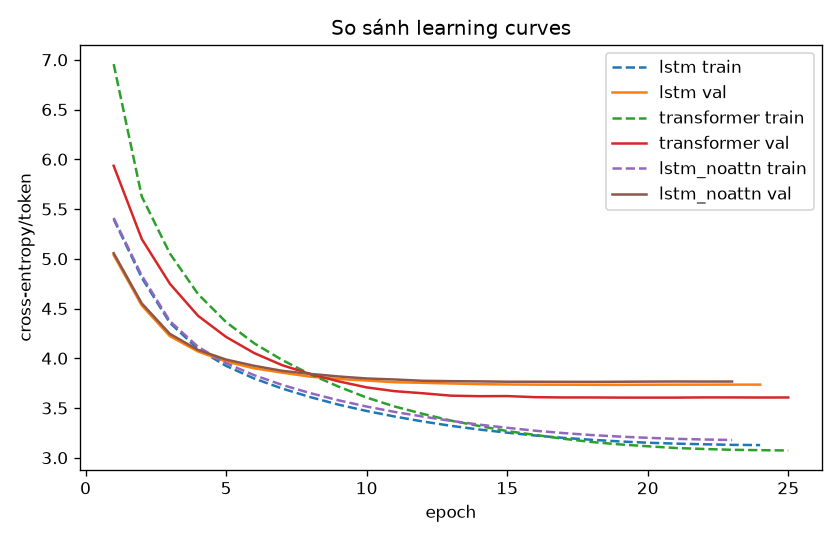
\includegraphics[width=0.95\textwidth]{figs/results/curves_main.png}
	\caption{Đường cong cross-entropy/token trên tập huấn luyện (nét đứt) và
	kiểm định (nét liền) của ba run chính, cùng seed 42. Transformer xuất phát
	cao hơn hẳn và chỉ vượt xuống dưới hai run LSTM quanh epoch 8--9, đúng vùng
	warmup 2.000 bước kết thúc.}
	\label{fig:curves}
\end{figure}

Hình~\ref{fig:curves} cho thấy ba điểm đáng bàn.

\textbf{Tốc độ hội tụ và dấu vết của warmup.} LSTM giảm loss rất nhanh trong
5 epoch đầu (train 5,40 $\to$ 3,92) rồi chậm dần; Transformer xuất phát cao hơn
hẳn (6,96) và giảm chậm trong giai đoạn đầu vì learning rate còn đang được nâng
dần theo lịch warmup. Với 30.000 mẫu và batch 128, một epoch có
$\approx$235 bước, nên 2.000 bước warmup tương đương $\approx$\textbf{8,5 epoch}
--- khớp chính xác với vị trí trên đồ thị nơi đường train của Transformer cắt
xuống dưới hai đường LSTM (epoch 8--9). Nói cách khác, gần một phần ba quá trình
huấn luyện của Transformer là ``chạy đà''; đây là cái giá về lịch huấn luyện đã
nêu ở mục 3.5, và cũng là lý do các caption mẫu của nó ``trưởng thành'' muộn
hơn (bảng~\ref{tab:samples-by-epoch}).

\textbf{Khoảng cách train--val: overfit nhẹ, được early stopping chặn đúng lúc.}
Cuối huấn luyện, khoảng cách train--val là 0,61 (LSTM), 0,53 (Transformer), 0,59
(không attention) --- có overfit nhưng ở mức lành: val loss của cả ba run
\emph{đi ngang} (plateau) chứ không quay đầu tăng, ví dụ LSTM đạt đáy 3,732 ở
epoch 19 rồi dao động quanh 3,734 suốt 5 epoch sau đó, khiến patience 5 kích
hoạt ở epoch 24. Dropout 0,3, label smoothing 0,1 và weight decay 0,01 giữ cho
phần ghi nhớ tập huấn luyện không phá hỏng khả năng khái quát.

\textbf{Loss gần nhau không có nghĩa metric gần nhau.} Val loss của LSTM có và
không có attention chỉ chênh 0,03 (3,732 so với 3,763), nhưng CIDEr chênh tới
0,051 (greedy). Attention giúp nhiều nhất ở chính những bước dự đoán ``khó'' ---
từ nội dung xuất hiện thưa --- vốn đóng góp ít vào loss trung bình trên token
nhưng quyết định chất lượng cảm nhận của cả câu. Đây là lý do đồ án không dừng
ở loss mà đo cả BLEU/CIDEr và soi từng bản đồ attention.

\subsection{Caption ``trưởng thành'' qua các epoch}

Trong suốt huấn luyện, sau mỗi epoch hệ thống sinh caption (greedy) cho 3 ảnh
kiểm định cố định. Bảng~\ref{tab:samples-by-epoch} trích ba mốc cho hai ảnh
tiêu biểu.

\begin{table}[H]
	\centering
	\caption{Caption greedy của cùng hai ảnh kiểm định qua các epoch (trích từ
	\texttt{samples\_by\_epoch.md}). Ảnh A: người leo trên mỏm đá; ảnh B: chó
	vượt rào trong sân thi đấu.}
	\label{tab:samples-by-epoch}
	\small
	\begin{tabular}{clp{4.6cm}p{4.6cm}}
		\hline
		\textbf{Epoch} & \textbf{Mô hình} & \textbf{Ảnh A} & \textbf{Ảnh B} \\
		\hline
		1  & LSTM        & a man in a a a a a & a dog dog dog a a a \\
		1  & Transformer & a a a a a a a a a a a a & a a a a a a a a a a a \\
		\hline
		5  & LSTM        & a man in a red shirt is jumping on a rock & a woman and a woman and a white dog is jumping over a white fence \\
		5  & Transformer & a man is jumping on a rock & a dog is jumping on a red ball \\
		\hline
		cuối & LSTM        & a man in a black shirt is jumping on a rock in the woods & a woman in a white and white dog is jumping over a hurdle \\
		cuối & Transformer & a boy in a white shirt is jumping off a rock & a woman in a white shirt is running through a grassy field \\
		\hline
	\end{tabular}
\end{table}

Quỹ đạo ``trưởng thành'' hiện rõ và khác nhau giữa hai kiến trúc. Ở epoch~1,
LSTM đã bắt được khung cú pháp ``a man in a\ldots'' nhưng thoái hóa thành lặp
mạo từ; Transformer khi đó còn chưa thoát khỏi chuỗi toàn ``a'' --- learning
rate mới đi được nửa đường warmup. Các epoch 2--4 của Transformer đầy những vòng
lặp cụm (``a man in a man in a\ldots''), rồi \emph{bật} khá đột ngột quanh epoch
5--6 sang câu đúng ngữ pháp. Từ epoch $\approx$10 trở đi, thay đổi chủ yếu là
tinh chỉnh chi tiết (màu áo đổi giữa black/white, thêm bối cảnh ``in the
woods'') --- nhất quán với đoạn plateau của val loss. Đáng chú ý, caption cuối
của LSTM cho ảnh B vẫn giữ một lỗi cấu trúc (``a woman in a white and white
dog'') trong khi Transformer cùng ảnh cho câu trôi chảy hơn --- một ví dụ nhỏ
cho thấy val loss thấp hơn của Transformer có thật ở mặt \emph{độ trôi chảy},
dù không đổi hết thành điểm BLEU.

\section{Phân tích định tính: attention nhìn đâu khi sinh từ}
\label{sec:qualitative}

Các hình dưới đây trực quan hóa trọng số attention khi decoder sinh từng từ:
với LSTM là trọng số Bahdanau (một đầu duy nhất), với Transformer là
cross-attention tầng cuối, trung bình 8 đầu; lưới $7\times7$ được nội suy và
phủ màu lên ảnh gốc (đỏ = trọng số cao). Toàn bộ nhận xét dưới đây dựa trên
các bản đồ nhiệt sinh từ checkpoint thật trên ảnh tập kiểm tra.

\subsection{Ca thành công}

\begin{figure}[H]
	\centering
	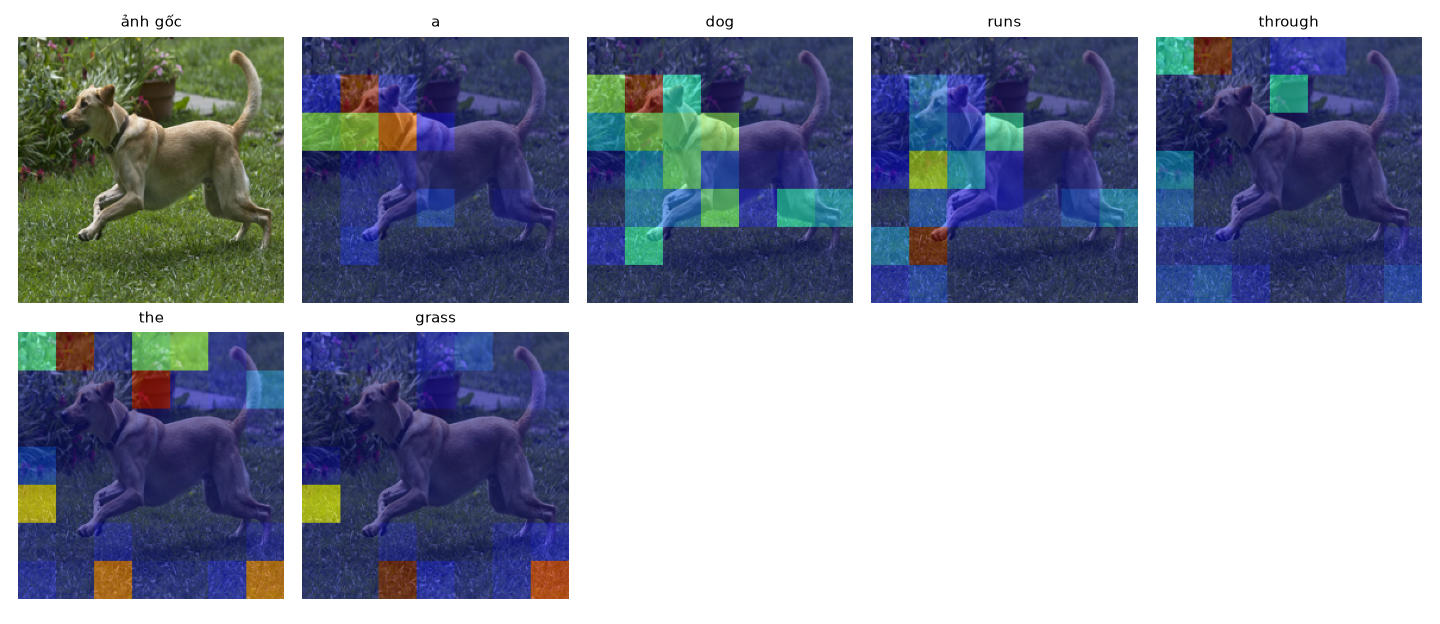
\includegraphics[width=0.88\textwidth]{figs/results/lstm_attention_5.png}
	\caption{LSTM+attention, ca thành công: ``a dog runs through the grass''.
	Khi sinh ``dog'', trọng số phủ lên thân chó; khi sinh ``grass'', vùng sáng
	rơi xuống các ô nền cỏ ở rìa dưới ảnh.}
	\label{fig:attn-success-lstm}
\end{figure}

\begin{figure}[H]
	\centering
	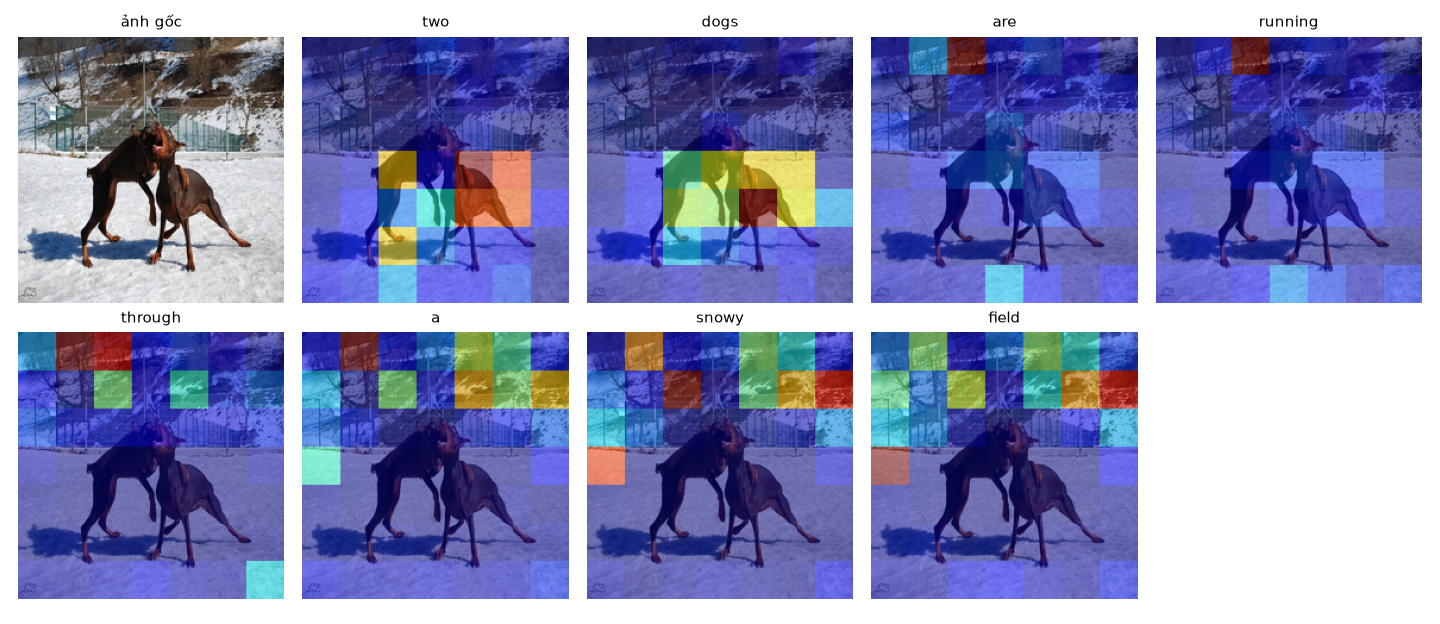
\includegraphics[width=0.88\textwidth]{figs/results/transformer_attention_0.png}
	\caption{Transformer, ca thành công: ``two dogs are running through a snowy
	field''. Khi sinh ``two'' và ``dogs'', dải trọng số trải ngang phủ \emph{cả
	hai} con chó; khi sinh ``snowy''/``field'', vùng sáng chuyển hẳn lên nền
	tuyết và sườn đồi phía sau.}
	\label{fig:attn-success-transformer}
\end{figure}

Ở hình~\ref{fig:attn-success-lstm}, hành vi của attention khớp trực giác ngôn
ngữ: từ nội dung bám vùng chứa vật thể (``dog'' $\to$ thân chó), từ chỉ bối
cảnh bám nền (``grass'' $\to$ các ô cỏ góc dưới), còn các từ chức năng
(``through'', ``the'') có bản đồ tản mát ra biên ảnh --- chúng được quyết định
bởi ngữ pháp của chuỗi đã sinh chứ không cần thông tin thị giác, nên mô hình
``nhìn đi chỗ khác'' cũng không sao. Hình~\ref{fig:attn-success-transformer}
còn thú vị hơn: đây là ảnh hai con chó chơi trên tuyết, và Transformer đếm
\emph{đúng} --- ``two dogs'' --- với dải attention phủ đồng thời cả hai con.

\subsection{Ca thất bại và chẩn đoán}

\begin{figure}[H]
	\centering
	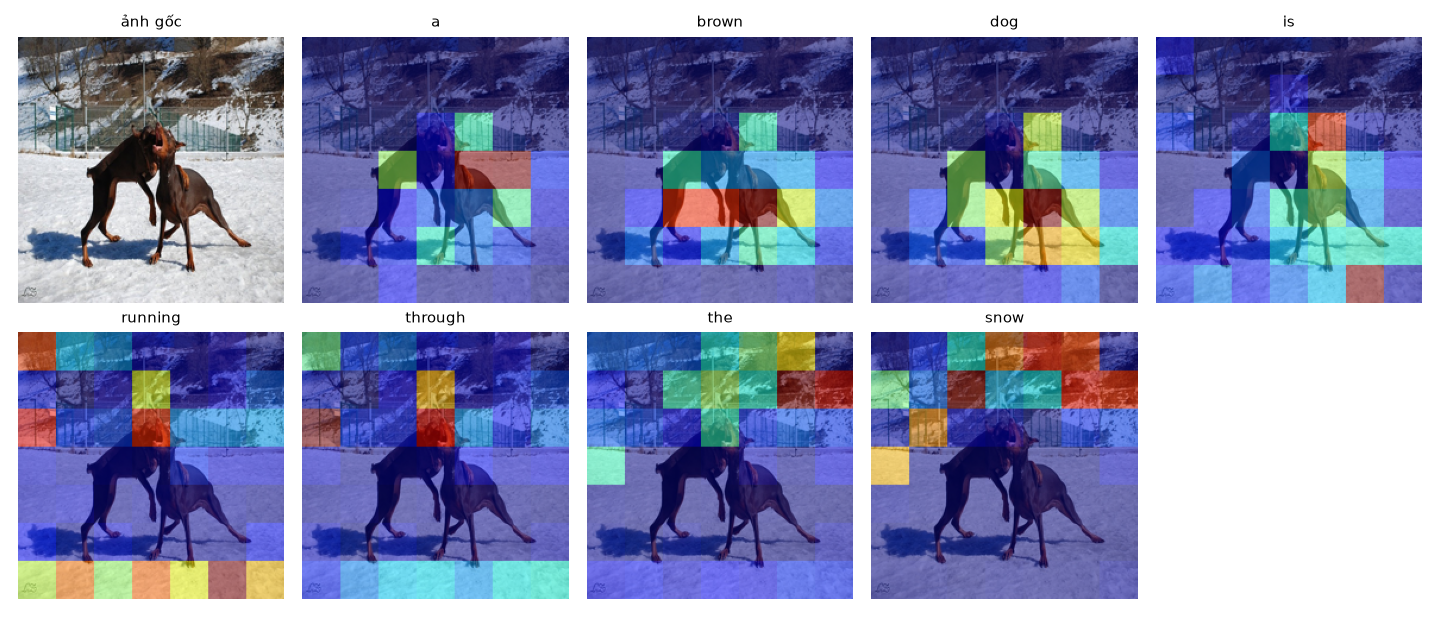
\includegraphics[width=0.88\textwidth]{figs/results/lstm_attention_0.png}
	\caption{LSTM+attention trên \emph{cùng ảnh} với
	hình~\ref{fig:attn-success-transformer}: ``a brown dog is running through
	the snow'' --- sai số đếm. Trọng số Bahdanau tạo đỉnh sắc, khóa vào một con
	chó (các ô đỏ tập trung ở con bên phải khi sinh ``dog'').}
	\label{fig:attn-fail-count}
\end{figure}

\begin{figure}[H]
	\centering
	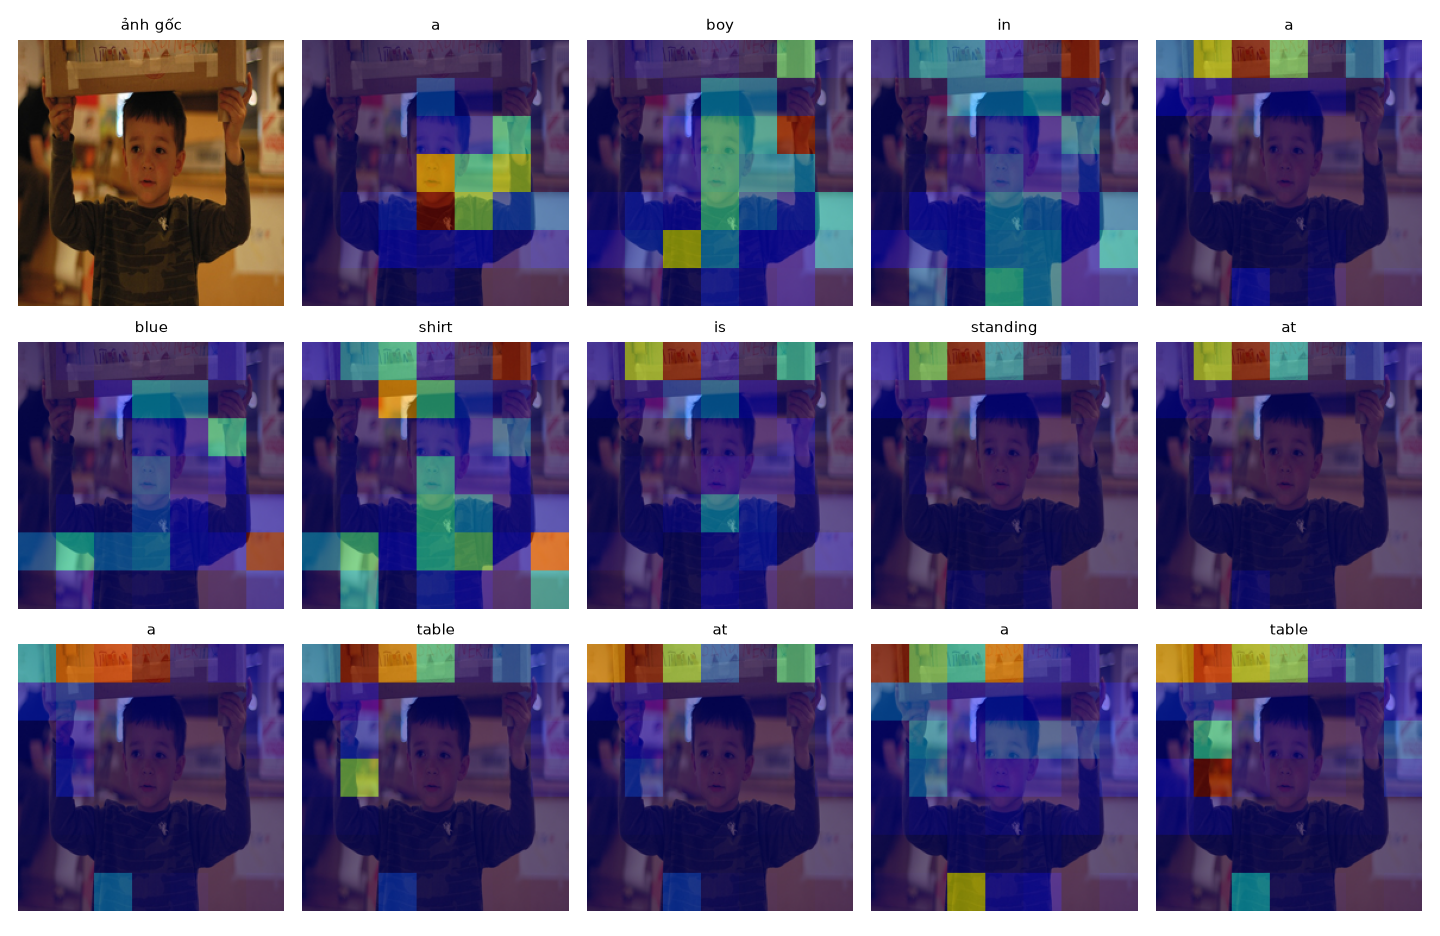
\includegraphics[width=0.88\textwidth]{figs/results/lstm_attention_17.png}
	\caption{LSTM+attention, ca thất bại kép: ``a boy in a blue shirt is
	standing at a table at a table''. Sai màu áo (áo rằn ri tối màu), lặp cụm
	``at a table'', nhưng khi sinh ``table'' attention trỏ đúng vào vật gỗ cậu
	bé đang nâng trên đầu.}
	\label{fig:attn-fail-loop}
\end{figure}

\begin{figure}[H]
	\centering
	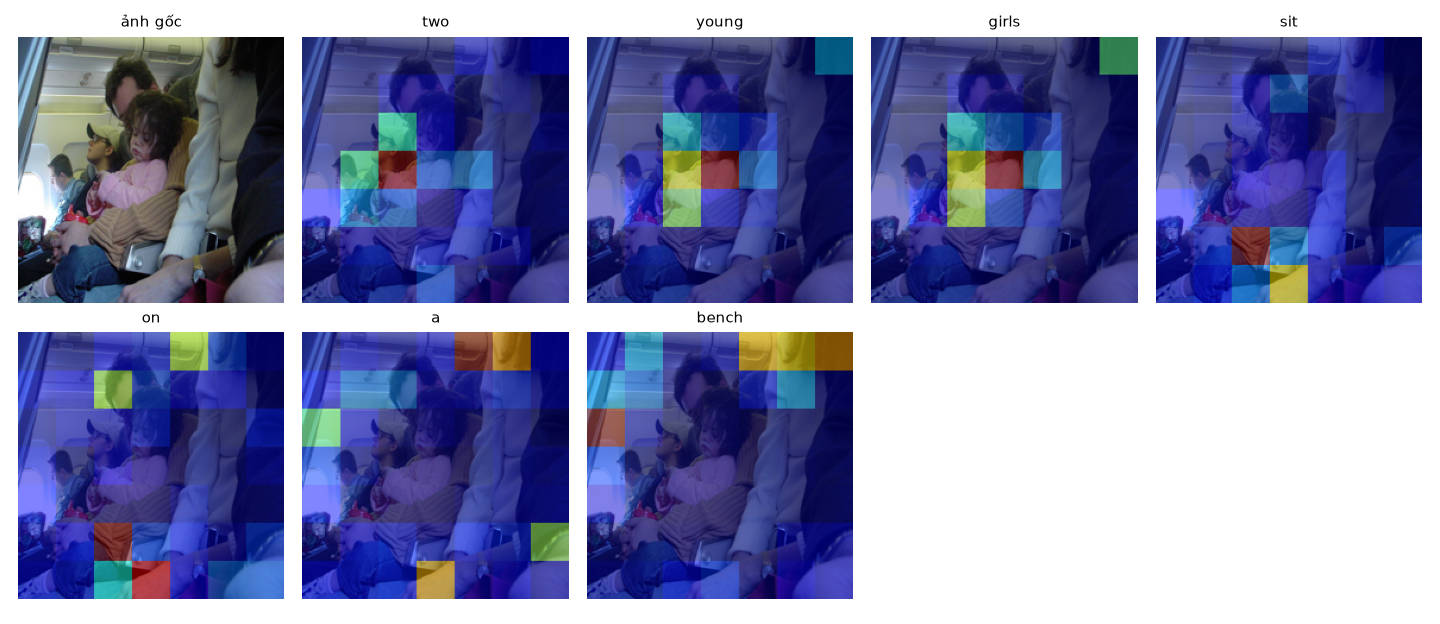
\includegraphics[width=0.88\textwidth]{figs/results/transformer_attention_42.png}
	\caption{Transformer, cảnh ngoài phân phối (khoang máy bay): ``two young
	girls sit on a bench''. Attention khi sinh ``two''/``girls'' vẫn bám đúng
	cụm khuôn mặt hành khách, nhưng danh tính (người lớn + trẻ em) và vật thể
	(ghế máy bay) đều bị kéo về khái niệm quen thuộc của Flickr8k.}
	\label{fig:attn-fail-ood}
\end{figure}

Ba ca thất bại trên minh họa ba chế độ lỗi khác nhau:

\textbf{Sai số đếm (hình~\ref{fig:attn-fail-count}).} Trên cùng một ảnh hai con
chó, LSTM nói ``a brown dog'' còn Transformer nói ``two dogs''. Bản đồ nhiệt gợi
ý nguyên nhân cơ chế: trọng số Bahdanau một đầu có xu hướng tạo \emph{đỉnh sắc}
--- dồn phần lớn khối lượng vào một cụm ô liền kề --- nên vector ngữ cảnh mỗi
bước gần như chỉ mô tả một con vật; trong khi bản đồ trung bình 8 đầu của
Transformer \emph{mượt và lan rộng hơn}, phủ cả hai con cùng lúc, đưa được tín
hiệu ``có nhiều hơn một'' vào decoder. Một đầu attention chỉ tạo ra một phân
phối trên 49 vùng mỗi bước; tám đầu được phép nhìn tám nơi rồi trộn lại --- với
bài toán đếm, đó là khác biệt về chất.

\textbf{Vòng lặp greedy và thuộc tính sai (hình~\ref{fig:attn-fail-loop}).}
Câu ``\ldots at a table at a table'' là thất bại của \emph{giải mã} chứ không
hẳn của attention: greedy không có cơ chế phạt lặp, và khi phân phối xác suất
tại một bước gần như dừng ở trạng thái cũ, chuỗi rơi vào chu trình. Điều đáng
ghi nhận là khi sinh ``table'', attention trỏ \emph{đúng} vào vật gỗ trên đầu
cậu bé --- mô hình nhìn đúng chỗ nhưng gọi tên sai, vì tư thế ``đội đồ gỗ trên
đầu'' gần như không tồn tại trong 30.000 caption huấn luyện; ``table'' là từ
gỗ-có-mặt-phẳng gần nhất mà từ điển của nó cung cấp. Màu áo ``blue'' cũng vậy:
áo rằn ri tối màu nằm ngoài bảng màu quần áo quen thuộc của dữ liệu.

\textbf{Cảnh ngoài phân phối (hình~\ref{fig:attn-fail-ood}).} Flickr8k hầu như
không có ảnh trong khoang máy bay, nên cả hai mô hình đều ``dịch'' cảnh lạ về
từ vựng quen: Transformer biến hành khách thành ``two young girls'' và ghế máy
bay thành ``bench'' (LSTM trên cùng ảnh còn kém hơn: ``a woman and woman sit on
a table''). Đây là dạng hallucination có hệ thống --- không phải nhìn nhầm
ngẫu nhiên mà là chiếu cảnh chưa từng gặp lên khái niệm gần nhất trong phân
phối huấn luyện --- và là lời nhắc rằng metric trung bình trên tập kiểm tra
cùng phân phối không nói gì về hành vi ngoài phân phối.

\textbf{So sánh hai cơ chế attention.} Nhìn xuyên suốt các hình: bản đồ Bahdanau
một đầu tương phản mạnh, ít ô rất sáng trên nền tối --- dễ đọc, ``chỉ tay'' rõ,
nhưng chính tính chọn lọc đó gây lỗi đếm; bản đồ trung bình 8 đầu của
Transformer mượt và loang hơn (nhiều ô mức trung bình), phần vì mỗi đầu nhìn
một nơi và phép trung bình làm nhòe các đỉnh riêng lẻ. Cả hai đều chung một
hành vi ở từ chức năng (``is'', ``a'', ``the''): trọng số tản ra biên hoặc nền,
xác nhận rằng attention chỉ thực sự ``làm việc'' ở những từ cần thông tin thị
giác.

\section{Phát hiện trong quá trình phát triển: thang khởi tạo embedding khi tie weight}
\label{sec:embedding-init}

Mục này ghi lại một lỗi thực tế gặp phải trong quá trình phát triển và cách xử
lý --- không phải kết quả thí nghiệm chính, nhưng là phát hiện có giá trị
phương pháp luận: so sánh công bằng hai kiến trúc đòi hỏi kiểm soát cả những
chi tiết ``ngầm định'' như thang khởi tạo tham số, không chỉ kiến trúc trên
giấy.

\subsection{Triệu chứng: cross-entropy ban đầu bất thường}

Trong lần \emph{smoke run} đầu tiên (512 mẫu, 2 epoch, trước khi có bất kỳ
bước huấn luyện nào tác động), cross-entropy đo ở batch đầu tiên của hai
decoder lệch nhau rất xa: LSTM+Bahdanau khoảng \textbf{13,0}, trong khi
Transformer khoảng \textbf{267,6}. Với $V = 2.539$ và nhãn được làm mượt (label
smoothing $0{,}1$), cross-entropy của một mô hình \emph{chưa học gì} --- tương
đương đoán gần như đều trên $V$ lớp --- được kỳ vọng xấp xỉ
\begin{equation}
	\text{CE}_{\text{kỳ vọng}} \approx \ln V + \text{(hiệu chỉnh nhỏ do
	smoothing)} \approx \ln(2.539) \approx 7{,}84 \;\Rightarrow\; \approx 7{,}9.
\end{equation}
Cả hai con số quan sát được (13,0 và 267,6) đều cao hơn hẳn mức kỳ vọng này,
và mức chênh giữa hai kiến trúc (LSTM lệch nhẹ, Transformer lệch gần 34 lần)
cho thấy nguyên nhân không phải ngẫu nhiên mà nằm ở một khác biệt hệ thống
giữa hai cách cài đặt.

\subsection{Nguyên nhân: weight tying nhân cái khởi tạo mặc định lên logits}

Cả hai decoder tie trọng số embedding với tầng đầu ra
(\S\ref{sec:decoder-detail}): $\text{logits} = h\,E^\top$, với $E \in
\mathbb{R}^{V\times D}$ là chính ma trận embedding. \texttt{torch.nn.Embedding}
mặc định khởi tạo $E \sim \mathcal{N}(0,1)$ --- một lựa chọn hợp lý \emph{nếu}
embedding chỉ dùng để tra cứu, nhưng có hại khi $E$ đồng thời là ma trận chiếu
ra logits.

Với Transformer, kiến trúc pre-norm đưa $h$ qua $\text{LN}_{\text{final}}$
ngay trước khi nhân với $E^\top$ (công thức cuối
mục~\ref{sec:decoder-detail}). LayerNorm chuẩn hoá mỗi vector $h$ về trung
bình 0, phương sai 1 trên $D$ chiều, tức mỗi thành phần $h_j \sim
\mathcal{O}(1)$. Với $E$ khởi tạo $\mathcal{N}(0,1)$, mỗi thành phần $E_{i,j}$
cũng $\mathcal{O}(1)$ và độc lập với $h$, nên với mỗi từ $i$:
\begin{align}
	\text{Var}(\text{logit}_i) &= \text{Var}\Big(\sum_{j=1}^{D} h_j E_{i,j}\Big)
	\approx D \cdot \text{Var}(h_j)\cdot\text{Var}(E_{i,j}) \approx D, \\
	\text{std}(\text{logit}_i) &\approx \sqrt{D} = \sqrt{512} \approx 22{,}6.
\end{align}
Logits có độ lệch chuẩn $\approx 22,6$ thay vì $\mathcal{O}(1)$ khiến phân phối
softmax gần như one-hot \emph{ngẫu nhiên} (không phải one-hot đúng nhãn) ---
cross-entropy trung bình bùng nổ, đúng như quan sát $267,6 \gg 7,9$. LSTM ít bị
ảnh hưởng hơn nhiều vì $h_t$ ở đây là trạng thái ẩn của \texttt{LSTMCell}, đi
qua các cổng sigmoid và $\tanh$ --- biên độ mỗi thành phần bị nén về khoảng
$(-1,1)$ với phương sai thực tế nhỏ hơn 1 khá nhiều (không có LayerNorm chuẩn
hoá về đúng phương sai 1 như phía Transformer), nên $\text{std}(\text{logit})$
tuy vẫn lớn hơn bình thường nhưng không bùng nổ theo $\sqrt{D}$ --- khớp với
mức lệch nhẹ hơn nhiều (13,0 so với 267,6).

\subsection{Giải pháp và kết quả sau khi sửa}

Sửa bằng cách khởi tạo embedding (và positional embedding của Transformer)
theo kiểu GPT-2/BERT: $E \sim \mathcal{N}(0,\,0{,}02^2)$ thay vì
$\mathcal{N}(0,1)$, đồng thời gán 0 cho hàng ứng với \texttt{<pad>} ngay tại
lúc khởi tạo (để token đệm không mang thông tin giả trước khi có gradient nào
chạy qua). Sau khi sửa, cross-entropy tại đầu smoke run của cả hai decoder hội
tụ đúng về vùng kỳ vọng: LSTM $\approx 7{,}84$, Transformer $\approx 7{,}95$ ---
sai khác nhỏ còn lại đến từ các tầng khác (dropout, chiếu ảnh) chứ không còn
do thang khởi tạo embedding. Cả hai sau đó giảm đều qua các epoch của smoke
run (2 epoch, 512 mẫu): LSTM $7{,}53 \to 6{,}71$; Transformer $7{,}93 \to
7{,}90$ --- xác nhận gradient chảy đúng hướng, không còn hiện tượng bùng nổ ở
bước đầu.

\subsection{Bài học}

So sánh công bằng hai kiến trúc (mục tiêu chính của đồ án, \S3.3) không chỉ
đòi hỏi giữ cố định các siêu tham số hiển thị (seed, batch size, optimizer)
mà còn cả những chi tiết ``ngầm định'' nằm sâu trong cách PyTorch khởi tạo
tầng mặc định --- ở đây là thang khởi tạo của embedding khi nó được tie với
tầng đầu ra \autocite{press2017using}. Một kiến trúc (Transformer, do có
LayerNorm cuối theo kiểu pre-norm \autocite{vaswani2017attention}) có thể lộ
lỗi rõ ràng hơn kiến trúc kia dù cả hai cùng mắc lỗi như nhau, khiến việc chẩn
đoán dễ quy nhầm cho ``Transformer khó train hơn'' thay vì đúng nguyên nhân kỹ
thuật. Hai unit test hồi quy
(\texttt{test\_embedding\_init\_nho\_khi\_tie\_weight} ở cả
\texttt{test\_lstm\_decoder.py} và \texttt{test\_transformer\_decoder.py})
được thêm ngay sau khi sửa để khóa lại bất biến này --- kiểm tra độ lệch chuẩn
của bảng embedding đủ nhỏ ($< 0,1$) và hàng \texttt{<pad>} bằng 0 tại lúc khởi
tạo, tránh lỗi tái diễn nếu decoder được viết lại sau này.

\section{Mở rộng: tinh chỉnh bằng SCST}
\label{sec:scst-results}

Giai đoạn mở rộng áp dụng Self-Critical Sequence Training
\autocite{rennie2017self} lên checkpoint LSTM+attention tốt nhất: 3 epoch,
phần thưởng CIDEr, baseline là điểm của chính câu giải mã greedy (mục 3.5).
Trong suốt 3 epoch, CIDEr greedy đo trên tập huấn luyện ổn định quanh
$\approx$1,27 --- phần thưởng không còn tăng thêm, cho thấy chính sách đã bão
hòa quanh một cực trị địa phương của reward.

\begin{table}[H]
	\centering
	\caption{SFT (LSTM+attention) so với sau tinh chỉnh SCST, tập kiểm tra
	1.000 ảnh.}
	\label{tab:scst}
	\begin{tabular}{llccccc}
		\hline
		\textbf{Mô hình} & \textbf{Giải mã} & \textbf{B-1} & \textbf{B-2} & \textbf{B-3} & \textbf{B-4} & \textbf{CIDEr} \\
		\hline
		SFT   & greedy & 0,624 & 0,447 & 0,306 & 0,203 & 0,536 \\
		+SCST & greedy & 0,630 & 0,454 & 0,312 & 0,208 & 0,546 \\
		\hline
		SFT   & beam 3 & 0,623 & 0,451 & 0,315 & 0,215 & 0,570 \\
		+SCST & beam 3 & 0,629 & 0,456 & 0,318 & 0,217 & 0,571 \\
		\hline
		SFT   & beam 5 & 0,625 & 0,453 & 0,319 & 0,219 & 0,573 \\
		+SCST & beam 5 & 0,629 & 0,457 & 0,322 & 0,221 & 0,575 \\
		\hline
	\end{tabular}
\end{table}

\textbf{Được gì.} Lợi ích rõ nhất nằm đúng nơi cơ chế self-critical nhắm tới:
giải mã \emph{greedy}, với CIDEr $+0{,}010$ (0,536 $\to$ 0,546) và mọi BLEU đều
nhích lên (B-1 0,630 --- cao nhất toàn bảng~\ref{tab:main-results}). Điều này
không ngẫu nhiên: trong SCST, gradient có dấu dương khi câu lấy mẫu tốt hơn câu
greedy của \emph{chính mô hình hiện tại} --- tức mô hình được huấn luyện trực
tiếp để ``câu greedy của tôi phải khó bị vượt qua''. SCST vì vậy là cách nâng
chất lượng ở chế độ suy luận rẻ nhất (greedy, không cần giữ $B$ giả thuyết),
hữu ích khi triển khai có ràng buộc độ trễ.

\textbf{Mất gì.} Khi đã dùng beam search, biên lợi gần như biến mất: beam 3 chỉ
còn $+0{,}001$ CIDEr, beam 5 còn $+0{,}002$. Beam search vốn đã ``vớt lại'' phần
lớn khoảng cách giữa greedy và tiềm năng của phân phối đã học, nên hai kỹ thuật
này chồng lấn nhau về lợi ích. Trong khi đó, chi phí mỗi bước SCST cao hơn hẳn
teacher forcing: phải lấy mẫu trọn câu, giải mã greedy trọn câu, rồi chấm CIDEr
cho từng mẫu trong batch. Với hệ có sẵn beam search, 3 epoch SCST trên bộ dữ
liệu này là một khoản đầu tư lợi suất thấp --- kết luận thực nghiệm quan trọng
không kém một cải thiện lớn.

\textbf{Khoảng cách reward train--test.} CIDEr greedy trên tập huấn luyện đạt
$\approx$1,27 trong khi trên tập kiểm tra chỉ 0,546. Một phần là overfitting
thông thường (mô hình đã học thuộc phong cách 5 câu tham chiếu của chính ảnh
huấn luyện --- các cụm n-gram TF--IDF cao dễ khớp lại), một phần là bản chất
của tối ưu reward: chính sách được đẩy về những mẫu câu ăn điểm CIDEr trên phân
phối tham chiếu \emph{đã thấy}, và lợi thế đó không chuyển hết sang ảnh mới.
Khoảng cách hơn hai lần này là lời nhắc rằng số đo reward trên train của một
vòng RL không phải là ước lượng chất lượng --- chỉ có tập kiểm tra giữ kín mới
trả lời được.

\section{Thí nghiệm mở rộng: kiểm tra độ vững của kết luận}
\label{sec:ext}

Mọi kết quả phía trên đều đến từ \emph{một} lần chạy (seed 42) với một lịch
warmup cố định --- hai chi tiết đủ sức làm lệch một so sánh sát nút như
LSTM--Transformer. Trước khi chốt kết luận, chúng tôi dùng quỹ máy còn lại để
trả lời bốn câu hỏi về độ vững: (i) khoảng cách giữa hai kiến trúc có phải
artifact của lịch warmup không; (ii) nó có lớn hơn nhiễu seed không; (iii)
đường cong theo beam bão hòa ở đâu; (iv) lợi ích của SCST có phụ thuộc kiến
trúc không. Các đánh giá trong mục này bổ sung thêm ROUGE-L
\autocite{lin2004rouge} --- F-measure trên chuỗi con chung dài nhất giữa câu
sinh và tham chiếu --- bên cạnh BLEU và CIDEr.

\subsection{Lịch warmup không phải thủ phạm}

Ghi chú ở mục~\ref{sec:learning-process} rằng warmup 2.000 bước chiếm tới
$\approx$8,5 epoch đặt ra nghi vấn: phải chăng Transformer ``thua thiệt'' vì
mất một phần ba thời gian huấn luyện chỉ để khởi động? Chúng tôi huấn luyện lại
Transformer với warmup 500 và 1.000 bước, giữ nguyên mọi siêu tham số khác.

\begin{table}[H]
	\centering
	\caption{Transformer theo số bước warmup, giải mã beam 3, tập kiểm tra
	1.000 ảnh.}
	\label{tab:warmup-sweep}
	\begin{tabular}{lcccc}
		\hline
		\textbf{Warmup} & \textbf{Val loss tốt nhất} & \textbf{B-4} & \textbf{ROUGE-L} & \textbf{CIDEr} \\
		\hline
		500   & 3,603 & 0,216 & 0,473 & 0,587 \\
		1.000 & 3,603 & 0,215 & 0,471 & 0,583 \\
		2.000 & 3,596 & 0,219 & 0,474 & 0,587 \\
		\hline
	\end{tabular}
\end{table}

Kết quả phẳng đến mức đáng ngạc nhiên: CIDEr dao động trong $[0{,}583;
0{,}587]$ và val loss lệch nhau 0,007 --- nhỏ hơn nhiễu giữa hai seed (bảng
dưới). Warmup ngắn hơn bốn lần không mở khóa thêm chất lượng nào: Transformer
đã đạt trần của nó trên Flickr8k, và trần đó không phải do lịch học suất đặt ra.

\subsection{Ba seed: hòa CIDEr trong nhiễu, LSTM vượt rõ ROUGE-L}

Chúng tôi huấn luyện lại cả hai mô hình chính với seed 43 và 44 (giữ nguyên
mọi thứ khác; seed 42 là run gốc), thu được trung bình $\pm$ độ lệch chuẩn trên
ba lần chạy độc lập.

\begin{table}[H]
	\centering
	\caption{Trung bình $\pm$ độ lệch chuẩn trên 3 seed (42/43/44), tập kiểm
	tra 1.000 ảnh.}
	\label{tab:seeds}
	\begin{tabular}{llccc}
		\hline
		\textbf{Mô hình} & \textbf{Giải mã} & \textbf{B-4} & \textbf{ROUGE-L} & \textbf{CIDEr} \\
		\hline
		LSTM+attention & greedy & 0,209 $\pm$ 0,004 & 0,471 $\pm$ 0,002 & 0,543 $\pm$ 0,005 \\
		Transformer    & greedy & 0,204 $\pm$ 0,002 & 0,460 $\pm$ 0,001 & 0,540 $\pm$ 0,010 \\
		\hline
		LSTM+attention & beam 3 & 0,220 $\pm$ 0,003 & 0,481 $\pm$ 0,001 & 0,575 $\pm$ 0,004 \\
		Transformer    & beam 3 & 0,212 $\pm$ 0,005 & 0,469 $\pm$ 0,004 & 0,576 $\pm$ 0,011 \\
		\hline
		LSTM+attention & beam 5 & 0,221 $\pm$ 0,004 & 0,482 $\pm$ 0,001 & 0,578 $\pm$ 0,006 \\
		Transformer    & beam 5 & 0,211 $\pm$ 0,003 & 0,467 $\pm$ 0,001 & 0,572 $\pm$ 0,007 \\
		\hline
	\end{tabular}
\end{table}

Bảng này buộc phải đọc lại bảng~\ref{tab:main-results} một cách thận trọng
hơn. Về CIDEr, hai kiến trúc \emph{không phân biệt được}: 0,575--0,578 (LSTM)
so với 0,572--0,576 (Transformer), chênh lệch nhỏ hơn một độ lệch chuẩn. Con số
0,587 từng là ``CIDEr SFT cao nhất'' của Transformer seed 42 hóa ra nằm ở mép
trên của dải nhiễu $\pm 0{,}011$ --- một lần gieo xúc xắc đẹp, không phải ưu
thế kiến trúc. Đáng chú ý, nhiễu seed của Transformer lớn gấp đôi LSTM ở CIDEr
(0,010--0,011 so với 0,004--0,006): mô hình nhiều tham số hơn trên dữ liệu nhỏ
không chỉ không thắng mà còn \emph{kém ổn định hơn} giữa các lần chạy. Ngược
lại, ở BLEU-4 và đặc biệt ROUGE-L, LSTM dẫn trước với khoảng cách nhiều lần độ
lệch chuẩn (0,482 $\pm$ 0,001 so với 0,467 $\pm$ 0,001 ở beam 5) --- khác biệt
này là thật, không phải nhiễu. Nói cách khác, ở quy mô Flickr8k, LSTM+attention
là lựa chọn vừa tốt hơn (nhẹ, ổn định, vượt ROUGE-L/BLEU) vừa rẻ hơn 2,3 lần
tham số.

\subsection{Đường cong beam: hai kiến trúc bão hòa khác nhau}

Bảng chính chỉ có ba điểm giải mã (greedy, beam 3, beam 5); chúng tôi mở rộng
sang $k \in \{1, 3, 5, 8, 12\}$ trên hai checkpoint seed 42 (hình~\ref{fig:beam-curve};
$k{=}1$ trùng khớp greedy đến từng chữ số --- một kiểm chứng chéo miễn phí cho
cài đặt beam search).

\begin{figure}[H]
	\centering
	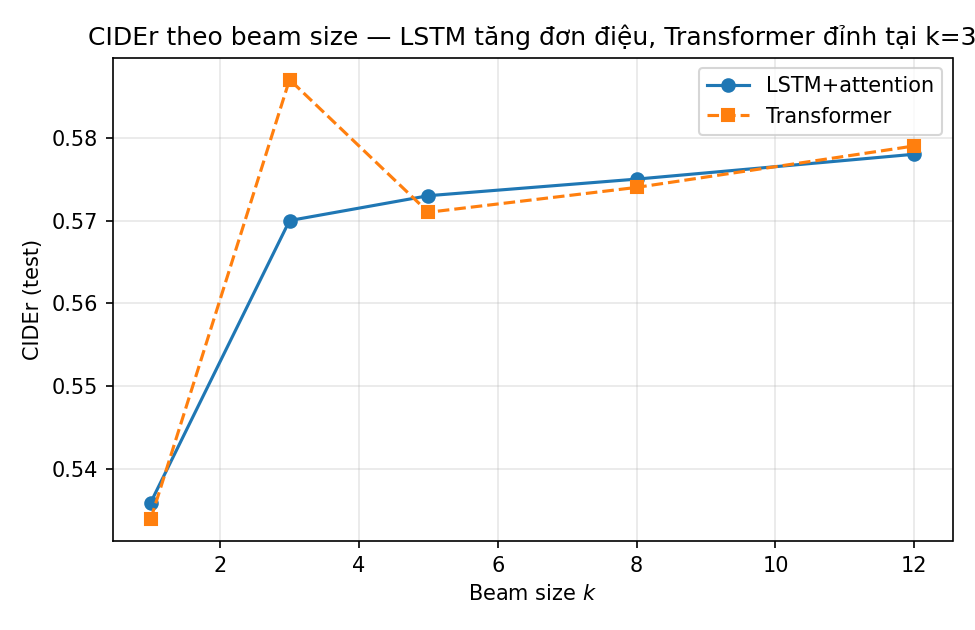
\includegraphics[width=0.8\textwidth]{figs/results/beam_curve.png}
	\caption{CIDEr trên tập kiểm tra theo beam size $k$. LSTM tăng đơn điệu
	và bão hòa dần; Transformer đạt đỉnh tại $k{=}3$ rồi tụt nhẹ.}
	\label{fig:beam-curve}
\end{figure}

Hai đường cong có hình dạng khác nhau về chất: LSTM tăng đơn điệu (0,536 ở
$k{=}1$ lên 0,578 ở $k{=}12$) và vẫn còn nhích ở $k{=}12$, trong khi
Transformer đạt đỉnh ngay tại $k{=}3$ (0,587) rồi dao động quanh 0,571--0,579.
Beam tối ưu là một siêu tham số \emph{theo kiến trúc}, không có giá trị đúng
chung. Một hệ quả thực dụng: LSTM ở beam 8 đạt BLEU-4 0,221 --- đúng bằng con
số tốt nhất mà SCST mang lại ở beam 5 --- nghĩa là chỉ cần tăng beam đã mua
được phần lớn lợi ích của cả một vòng tinh chỉnh RL, với chi phí suy luận thay
vì chi phí huấn luyện.

\subsection{SCST trên Transformer: lợi ích lặp lại, không phụ thuộc kiến trúc}

Mục~\ref{sec:scst-results} chỉ tinh chỉnh LSTM. Lặp lại đúng quy trình đó (3
epoch, phần thưởng CIDEr) trên checkpoint Transformer:

\begin{table}[H]
	\centering
	\caption{Transformer trước và sau SCST, tập kiểm tra 1.000 ảnh.}
	\label{tab:scst-transformer}
	\begin{tabular}{llccc}
		\hline
		\textbf{Mô hình} & \textbf{Giải mã} & \textbf{B-4} & \textbf{ROUGE-L} & \textbf{CIDEr} \\
		\hline
		SFT   & greedy & 0,207 & 0,460 & 0,534 \\
		+SCST & greedy & 0,211 & 0,469 & 0,547 \\
		\hline
		SFT   & beam 3 & 0,219 & 0,474 & 0,587 \\
		+SCST & beam 3 & 0,219 & 0,476 & 0,578 \\
		\hline
		SFT   & beam 5 & 0,215 & 0,469 & 0,571 \\
		+SCST & beam 5 & 0,217 & 0,476 & 0,582 \\
		\hline
	\end{tabular}
\end{table}

Bức tranh lặp lại gần như nguyên vẹn kết quả bên LSTM: greedy hưởng lợi nhiều
nhất (CIDEr $+0{,}013$, so với $+0{,}010$ bên LSTM), còn khi đã dùng beam thì
biên lợi mờ đi. Điểm ``tụt'' duy nhất --- beam 3 giảm từ 0,587 xuống 0,578 ---
không mâu thuẫn: 0,587 chính là điểm mép-trên-nhiễu đã bàn ở trên, và 0,578 sau
SCST nằm gọn trong dải $0{,}576 \pm 0{,}011$ của ba seed. Kết luận phương pháp:
lợi ích của SCST đến từ \emph{cơ chế} (kéo câu greedy về phía reward) chứ không
từ kiến trúc decoder, nên có thể kỳ vọng nó chuyển giao sang các decoder khác.

\subsection{Bảng chính, đọc lại}

Bốn thí nghiệm bổ sung không lật đổ kết luận nào nhưng đổi \emph{trọng âm} của
chúng: ``Transformer đạt CIDEr cao nhất'' (một lần chạy) trở thành ``hai kiến
trúc hòa CIDEr trong nhiễu seed, LSTM vượt có ý nghĩa ở ROUGE-L/BLEU với chi
phí 2,3 lần thấp hơn và độ ổn định giữa các lần chạy gấp đôi''. Đây là minh họa
cụ thể cho một nguyên tắc thực nghiệm: với các khác biệt cỡ 0,01, một lần chạy
không phải bằng chứng --- phải trả lời bằng nhiều seed và phân tích độ nhạy
trước khi tuyên bố người thắng.

\section{Bàn luận}

\begin{itemize}
	\item \textbf{LSTM và Transformer trên dữ liệu nhỏ:} với cùng ngân sách dữ
	      liệu (30.000 caption), Transformer \emph{không} thua như lo ngại ban
	      đầu --- val loss thấp nhất và CIDEr một lần chạy cao nhất (0,587,
	      beam 3) --- nhưng mục~\ref{sec:ext} cho thấy nó cũng \emph{không}
	      thắng: qua 3 seed, CIDEr của hai kiến trúc không phân biệt được,
	      LSTM còn vượt có ý nghĩa ở ROUGE-L/BLEU-4, trong khi Transformer trả
	      giá 2,3$\times$ tham số, nhiễu seed gấp đôi, và $\approx$8,5 epoch
	      warmup (dù sweep warmup xác nhận rút ngắn lịch cũng không đổi kết
	      quả). Ở quy mô này, thiên kiến quy nạp tuần tự của LSTM vẫn ``mua''
	      được gần trọn những gì attention đa đầu phải học từ dữ liệu; bài học
	      là lựa chọn kiến trúc phải đặt trong ngân sách dữ liệu--tham
	      số--lịch huấn luyện, không có người thắng tuyệt đối.
	\item \textbf{Attention đóng góp gì:} tắt attention làm CIDEr greedy giảm
	      10,5\% (0,536 $\to$ 0,485) --- khoảng cách lớn nhất giữa hai mô hình
	      cùng họ trong bảng chính, lớn hơn cả khác biệt LSTM/Transformer ---
	      và bản đồ nhiệt xác nhận cơ chế: từ nội dung bám đúng vùng vật thể,
	      từ bối cảnh bám nền. Đổi lấy mức tăng đó chỉ là 0,53 triệu tham số
	      của khối Bahdanau: tính theo ``CIDEr trên mỗi tham số thêm vào'',
	      attention là khoản đầu tư hiệu quả nhất toàn đồ án.
	\item \textbf{Đặt cạnh đồ án giữa kỳ:} Medical VQA (phân loại) và captioning
	      (sinh chuỗi) là hai nhánh đầu ra của cùng meta-kiến trúc đa phương thức;
	      điểm chung là khối fusion bằng attention, điểm khác là không gian đầu ra
	      --- nhãn rời rạc so với chuỗi mở. Kết quả hai đồ án phản chiếu đúng
	      khác biệt đó: ở VQA, mọi phức tạp dồn vào việc trộn hai phương thức
	      trước một quyết định duy nhất; ở captioning, chuỗi mở kéo theo cả một
	      tầng vấn đề mới không tồn tại bên phân loại --- chiến lược giải mã
	      (greedy/beam làm lệch CIDEr tới 0,053 trên \emph{cùng một} mô hình),
	      vòng lặp cụm từ, và khả năng tối ưu trực tiếp metric chuỗi bằng RL
	      (SCST). Nhìn từ trên xuống, ``đầu ra là gì'' quyết định phần lớn độ
	      khó kỹ thuật của một hệ đa phương thức, hơn cả việc hai phương thức
	      được trộn thế nào.
\end{itemize}
